\section{Anwenderdokumentation}



\subsection{Seitenerläuterung}

\subsubsection{Anmeldeseite}\label{Login}
\begin{figure}[H]
	\centering
	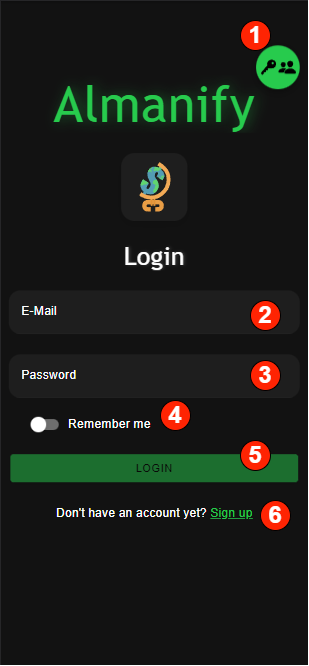
\includegraphics[width=0.3\textwidth]{img/pages_numbers/login.drawio}
	\caption[Login]{Login}
	%\captionsource{}
	\label{fig:Login}
\end{figure}

Auf dieser Seite kann sich der User anmelden.

\begin{enumerate}[label=\protect\circled{\arabic*}]
	\item Schnelllogin: ermöglicht das schnelle Anmelden mit verschiedenen Testuseren. (nur im Debugmodus vorhanden)
	\item Eingabefeld für die E-Mail-Adresse des Nutzers, mit der er sich registriert hat.
	\item Eingabefeld für das Passwort des Nutzers.
	\item \emph{Rememeber Me}: der User kann auswählen, ob er sich nach Schließen der App erneut anmelden möchte.
	\item Button um sich einzuloggen.
	\item Wenn der Nutzer noch keinen Account hat gelangt er hier zur Registrierungsseite (Siehe \ref{Signup}).
\end{enumerate}

\subsubsection{Registrierungsseite}\label{Signup}
\begin{figure}[H]
	\centering
	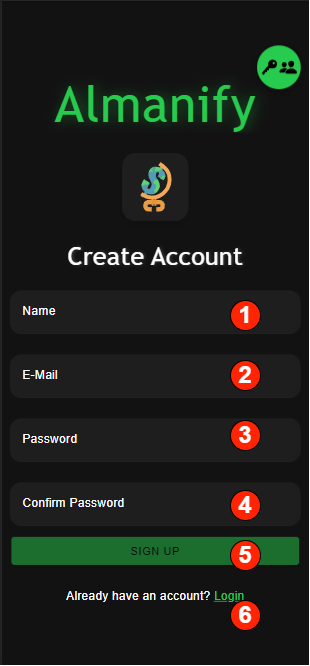
\includegraphics[width=0.3\textwidth]{img/pages_numbers/signup.drawio}
	\caption[Signup]{Signup}
	%\captionsource{}
	\label{fig:Signup}
\end{figure}

Auf dieser Seite kann sich der User registrieren.

\begin{enumerate}[label=\protect\circled{\arabic*}]
	\item Eingabefeld für den Nutzernamen, welcher den Mitreisenden später angezeigt wird.
	\item Eingabefeld für die E-Mail-Adresse des Nutzers.
	\item Eingabefeld für das Passwort des Nutzers.
	\item Eingabefeld um das Passwort des Nutzers zu bestätigen.
	\item Button um sich zu registrieren.
	\item Wenn der Nutzer einen Account hat gelangt er hier zurück zu Loginseite (Siehe \ref{Login}).
\end{enumerate}

\subsubsection{Home}\label{Home}
\begin{figure}[H]
	\centering
	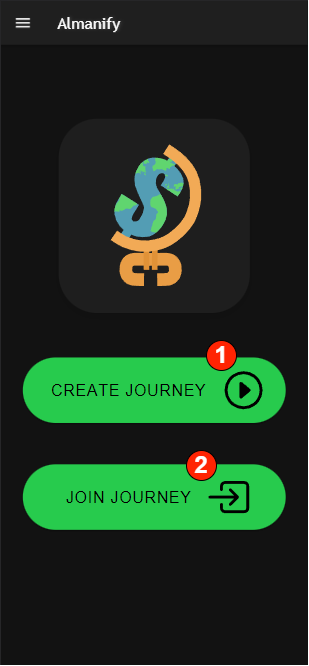
\includegraphics[width=0.3\textwidth]{img/pages_numbers/home.drawio}
	\caption[Home]{Home}
	%\captionsource{}
	\label{fig:Home}
\end{figure}

Auf diese Seite gelangt der User nach Login, wenn keine aktive Reise vorhanden ist.

\begin{enumerate}[label=\protect\circled{\arabic*}]
	\item Button zum Erstellen einer neuen Reise: der Nutzer gelangt zur Reiseerstellenseite (Siehe \ref{Journey-Editor}).
	\item Button zum Beitreten einer existierenden Reise: der Nutzer gelangt zur Reisebeitretenseite (Siehe [TODO]).
\end{enumerate}

\subsubsection{Reisebearbeiten/erstellen}\label{Journey-Editor}
\begin{figure}[H]
	\centering
	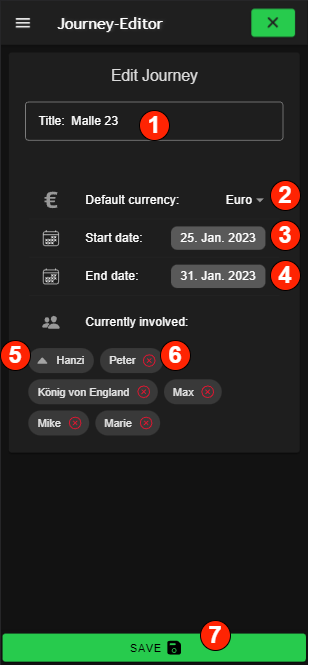
\includegraphics[width=0.3\textwidth]{img/pages_numbers/journey-editor.drawio}
	\caption[Journey-Editor]{Journey-Editor}
	%\captionsource{}
	\label{fig:Journey-Editor}
\end{figure}

Auf dieser Seite kann der User eine Reise erstellen oder bearbeiten. Entsprechend der Situation ist der Titel  "`New Journey"' oder "`Edit Journey"'.

\begin{enumerate}[label=\protect\circled{\arabic*}]
	\item Eingabefeld um der Reise einen Titel zugeben der später für alle Angezeigt wird.
	\item Dropdown zur Auswahl einer Standardwährung auf der Reise.
	      Die Standardwährung ist später beim Erstellen von Zahlungen voreingestellt.
	\item Öffnet Modal zur Wahl des Startdatums der Reise.
	\item Öffnet Modal zur Wahl des Enddatums der Reise.
	\item Ersteller einer Reise wird mit Dreieckicon markiert.
	\item Nicht-Ersteller einer Reise können mit x-Button aus der Reise gekickt werde.
	\item Button zum Speichern des Eintrags.
	\item Mit Dateiauswahl-Button kann der Reise ein Banner hinzugefügt werden. Das Banner wird dann in der Reiseliste angezeigt.
\end{enumerate}

\subsubsection{Detailansicht einer Reise}\label{Journey-Details}
\begin{figure}[H]
	\centering
	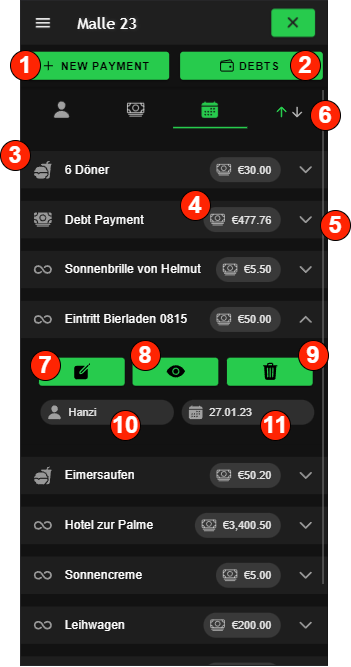
\includegraphics[width=0.3\textwidth]{img/pages_numbers/journey-details.drawio}
	\caption[Journey-Details]{Journey-Details}
	%\captionsource{}
	\label{fig:Journey-Details}
\end{figure}

Auf dieser Seite hat der Nutzer eine Übersicht aller Zahlungen einer Reise.
Der Nutzer gelangt nach Login auf diese Seite, wenn es sich um die aktuellste Reise handelt.

\begin{enumerate}[label=\protect\circled{\arabic*}]
	\item Button zum Erstellen einer neuen Zahlung: der Nutzer gelangt zur Zahlungerstellenseite (Siehe \ref{payment-details_(edit-mode)}).
	\item Button zur Schuldenübersicht: der Nutzer gelangt zu Schuldenübersicht der Reise (Siehe \ref{debt-calculator_(owe)} und \ref{debt-calculator_(owed)}).
	\item Icon sagt über Kategorie der Zahlung aus (siehe Tabelle \ref{Tab:paymentcategories}).
	\item Betrag und Währung einer Zahlung.
	\item Öffnen von weiteren Optionen zu einer Zahlung.
	\item Zahlung können auf- und absteigend anhand des Zahlers, des Betrags und des Zahldatums sortiert werden.
	\item Button zum Bearbeiten einer Zahlung: Der Nutzer gelangt zur Zahlungbearbeitenseite  (Siehe \ref{payment-details_(edit-mode)}).
	\item Button zu Details einer Ausgabe: Der Nutzer gelangt zur Detailansicht einer Zahlung  (Siehe \ref{payment-details}).
	\item Button zum Löschen einer Zahlung.
	\item Nutzername des Zahlers.
	\item Zahldatum.
\end{enumerate}

\begin{table}[H]
	\caption{Zahlungskategorien}
	\begin{tabularx}{0.95\textwidth}{ |X|X|X| }
		\hline
		\rowcolor{gray} \textbf{Bezeichnung} & \textbf{Icon}                                                                 & Beschreibung                                    \\
		\hline
		Accommodation                        & 
\includegraphics[width=0.05\textwidth]{paymentcategories/bed.pdf}             &
		Ausgaben für Unterkunft.                                                                                                                                               \\
		\hline
		Food and drink                          & 
\includegraphics[width=0.05\textwidth]{paymentcategories/fast-food.pdf}       & Ausgaben für Essen und Trinken.                 \\
		\hline
		Entertaiment                         & 
\includegraphics[width=0.05\textwidth]{paymentcategories/game-controller.pdf} & Ausgaben für Unterhaltung.                      \\
		\hline
		Transfer                             & 
\includegraphics[width=0.05\textwidth]{paymentcategories/airplane.pdf}        & Ausgaben die Transportmittel betreffen.         \\
		\hline
		Repayment                            & 
\includegraphics[width=0.05\textwidth]{paymentcategories/cash.pdf}            & Rückzahlung von Schulden an andere Mitreisende. \\
		\hline
		Other                                & 
\includegraphics[width=0.05\textwidth]{paymentcategories/infinite.pdf}        & Alles was in keine andere Kategorie passt.      \\
		\hline
	\end{tabularx}
	\label{Tab:paymentcategories}
\end{table}

\subsubsection{Liste der beigetretenen Reisen}\label{Journey-List}
\begin{figure}[H]
	\centering
	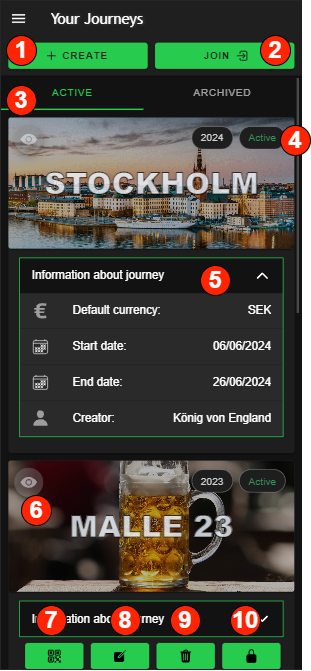
\includegraphics[width=0.3\textwidth]{img/pages_numbers/journey-list.drawio}
	\caption[Journey-List]{Journey-List}
	%\captionsource{}
	\label{fig:Journey-List}
\end{figure}

Auf dieser Seite hat der Nutzer eine Übersicht aller beigetretenen Reisen.

\begin{enumerate}[label=\protect\circled{\arabic*}]
	\item Button zum Erstellen einer neuen Reise: der Nutzer gelangt zur Reiseerstellenseite  (Siehe \ref{Journey-Editor}).
	\item Button zum Beitreten einer existierenden Reise: der Nutzer gelangt zur Reisebeitretenseite (Siehe [TODO]).
	\item Auswahl zwischen aktiven und archivierten Reisen.
	\item Anzeige, ob es sich um eine aktive oder archivierte Reise handelt.
	\item Dropdown mit allen wichtigen Infos zu einer Reise.
	\item Durch klicken auf das Reisebanner gelangt der Nutzer zu  den Details einer Reise: der Nutzer gelangt zu einer Listenansicht aller Reisezahlungen  (Siehe \ref{Journey-Details}). Das Banner kann vom Nutzer zu einem beliebigen Bild geändert werden.
	\item Der Nutzer bekommt das Einladungsmodal angezeigt (Siehe \ref{invite-modal}).*
	\item Button zum Reisebearbeiten: der Nutzer gelangt zur Reisebearbeitenseite (Siehe \ref{Journey-Editor}).*
	\item Button zum Löschen einer Reise.*
	\item Button zum Archivieren einer Reise.*
\end{enumerate}
* Werden dem Nutzer nur angezeigt, wenn dieser Ersteller der Reise ist.
\subsubsection{Details einer Zahlung}\label{payment-details}
\begin{figure}[H]
	\centering
	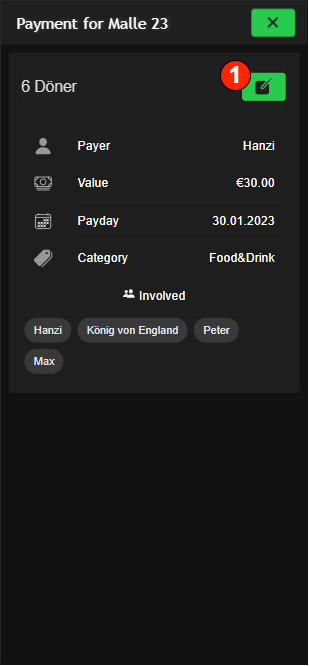
\includegraphics[width=0.3\textwidth]{img/pages_numbers/payment-details.drawio}
	\caption[Payment-Details]{Payment-Details}
	%\captionsource{}
	\label{fig:payment-details}
\end{figure}

Auf dieser Seite sieht der Nutzer alle Informationen zu einer Zahlung.

\begin{enumerate}[label=\protect\circled{\arabic*}]
	\item Wechseln in den Bearbeitenmodus (Siehe \ref{payment-details_(edit-mode)}).
\end{enumerate}

\subsubsection{Details einer Zahlung beim Erstellen/Bearbeiten}\label{payment-details_(edit-mode)}
\begin{figure}[H]
	\centering
	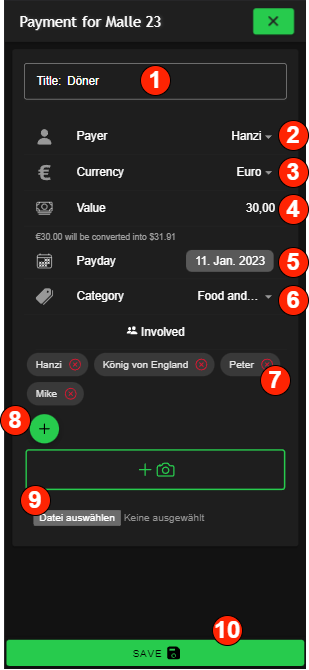
\includegraphics[width=0.3\textwidth]{img/pages_numbers/payment-details_(edit-mode).drawio}
	\caption[Payment-Details (Edit-Mode)]{Payment-Details (Edit-Mode)}
	%\captionsource{}
	\label{fig:payment-details_(edit-mode)}
\end{figure}

Auf dieser Seite kann der Nutzer die Informationen zu einer Zahlung erstellen oder bearbeiten.

\begin{enumerate}[label=\protect\circled{\arabic*}]
	\item Titel der Zahlung
	\item Dropdown mit allen Reisebeteiligten zur Auswahl des Zahlers. Der Ersteller einer Zahlung ist hier 			vorausgewählt.
	\item Dropdown für die Wahl der Währung. Die Standartwährung der Reise ist beim Erstellen vorausgewählt.
	\item Input für den Betrag der Zahlung.
	\item Öffnet Modal, um den Zahltag auszuwählen.
	\item Dropdown zur Auswahl der Zahlungskategorie.
	\item Durch den x-Button können Nutzer als Zahlungsverursacher entfernt werden.
	\item Mit dem Plus-Button können einzelne Nutzer oder alle Nutzer hinzugefügt werden. Zusätzlich gibt es die Möglichkeit alle Nutzer zu entfernen.
	\item Button um die Kamera zu öffnen und um ein Bild der Rechnung festzuhalten.
	Alternativ kann der Nutzer ein Bild aus der Galerie hochladen.
	\item Button zum Speichern des Eintrags.
\end{enumerate}


\subsubsection{Schuldenansicht bei Guthaben}\label{debt-calculator_(owed)}
\begin{figure}[H]
	\centering
	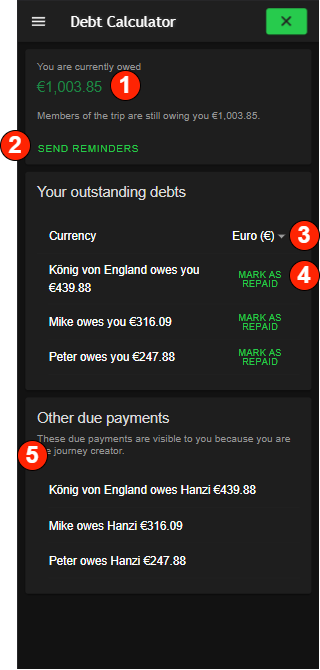
\includegraphics[width=0.3\textwidth]{img/pages_numbers/debt-calculator_(owed).drawio}
	\caption[Debt-Calculator (Owed)]{Debt-Calculator (Owed)}
	%\captionsource{}
	\label{fig:debt-calculator_(owed)}
\end{figure}
Auf dieser Seite sieht der Nutzer sein Guthaben bzw. seine Schulden gegenüber anderen (Siehe \ref{debt-calculator_(owe)}).
\begin{enumerate}[label=\protect\circled{\arabic*}]
	\item Der Betrag, was einem die Mitreisenden noch schulden.
	\item Sendet eine Push-Nachricht als Erinnerung an alle Schuldner.
	\item Dropdown zur Auswahl der Schuldenwährung.
	\item Öffnet Zahlung erstellen, um den gezahlten Betrag festzuhalten.
	\item Als Reiseersteller hat man zusätzlich die Übersicht über alle offene Schulden einer Reise.
\end{enumerate}

\subsubsection{Schuldenansicht bei Schulden}\label{debt-calculator_(owe)}
\begin{figure}[H]
	\centering
	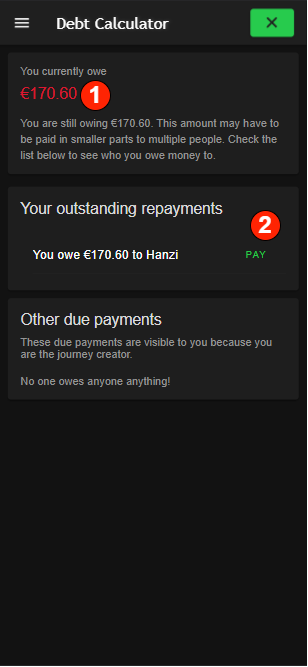
\includegraphics[width=0.3\textwidth]{img/pages_numbers/debt-calculator_(owe).drawio}
	\caption[Debt-Calculator (Owe)]{Debt-Calculator (Owe)}
	%\captionsource{}
	\label{fig:debt-calculator_(owe)}
\end{figure}
\begin{enumerate}[label=\protect\circled{\arabic*}]
	\item Der Betrag, was man den Mitreisenden noch schuldet.
	\item Dropdown zur Auswahl der Schuldenwährung.
	\item Öffnet Zahlung erstellen mit vor gefüllten Werten, um die Übermittlung einer Zahlung festzuhalten.
\end{enumerate}

\subsubsection{Einladungsmodal}\label{invite-modal}
\begin{figure}[H]
	\centering
	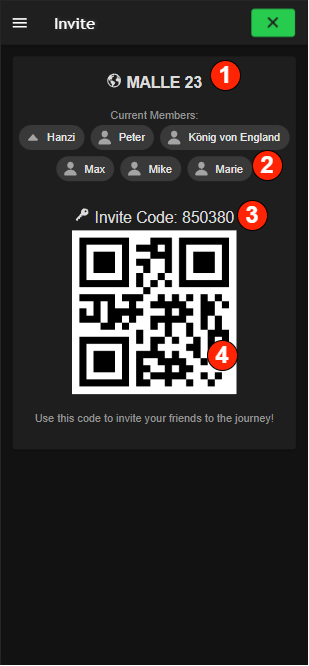
\includegraphics[width=0.3\textwidth]{img/pages_numbers/invite-modal.drawio}
	\caption[Invite-Modal]{Invite-Modal}
	%\captionsource{}
	\label{fig:invite-modal}
\end{figure}

Auf dieser Seite erhält der Reiseersteller alle Informationen, um weitere Nutzer in seine Reise einzuladen.

\begin{enumerate}[label=\protect\circled{\arabic*}]
	\item Title der Reise für die eingeladen wird.
	\item Liveansicht aller der Reise beigetretenen Nutzer.
	\item Invitecode zur Eingabe auf der Reisebeitrittseite um der Reise beizutreten.
	\item Der Invitecode als QR-Code zum einfachen Scannen auf der Reisebeitrittseite um der Reise beizutreten.
\end{enumerate}

\subsubsection{Optionen}\label{options}
\begin{figure}[H]
	\centering
	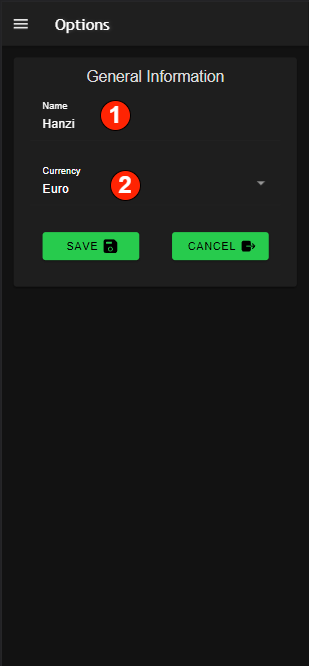
\includegraphics[width=0.3
		\textwidth]{img/pages_numbers/options.drawio}
	\caption[Options]{Options}
	%\captionsource{}
	\label{fig:options}
\end{figure}

Auf dieser Seite kann der Nutzer seine Daten anpassen.

\begin{enumerate}[label=\protect\circled{\arabic*}]
	\item Ändern des Nutzernamens.
	\item Anpassen der Wunschwährung in der Schulden angezeigt werden sollen.
\end{enumerate}


\subsection{Sitemap}

\begin{figure}[H]
	\centering
	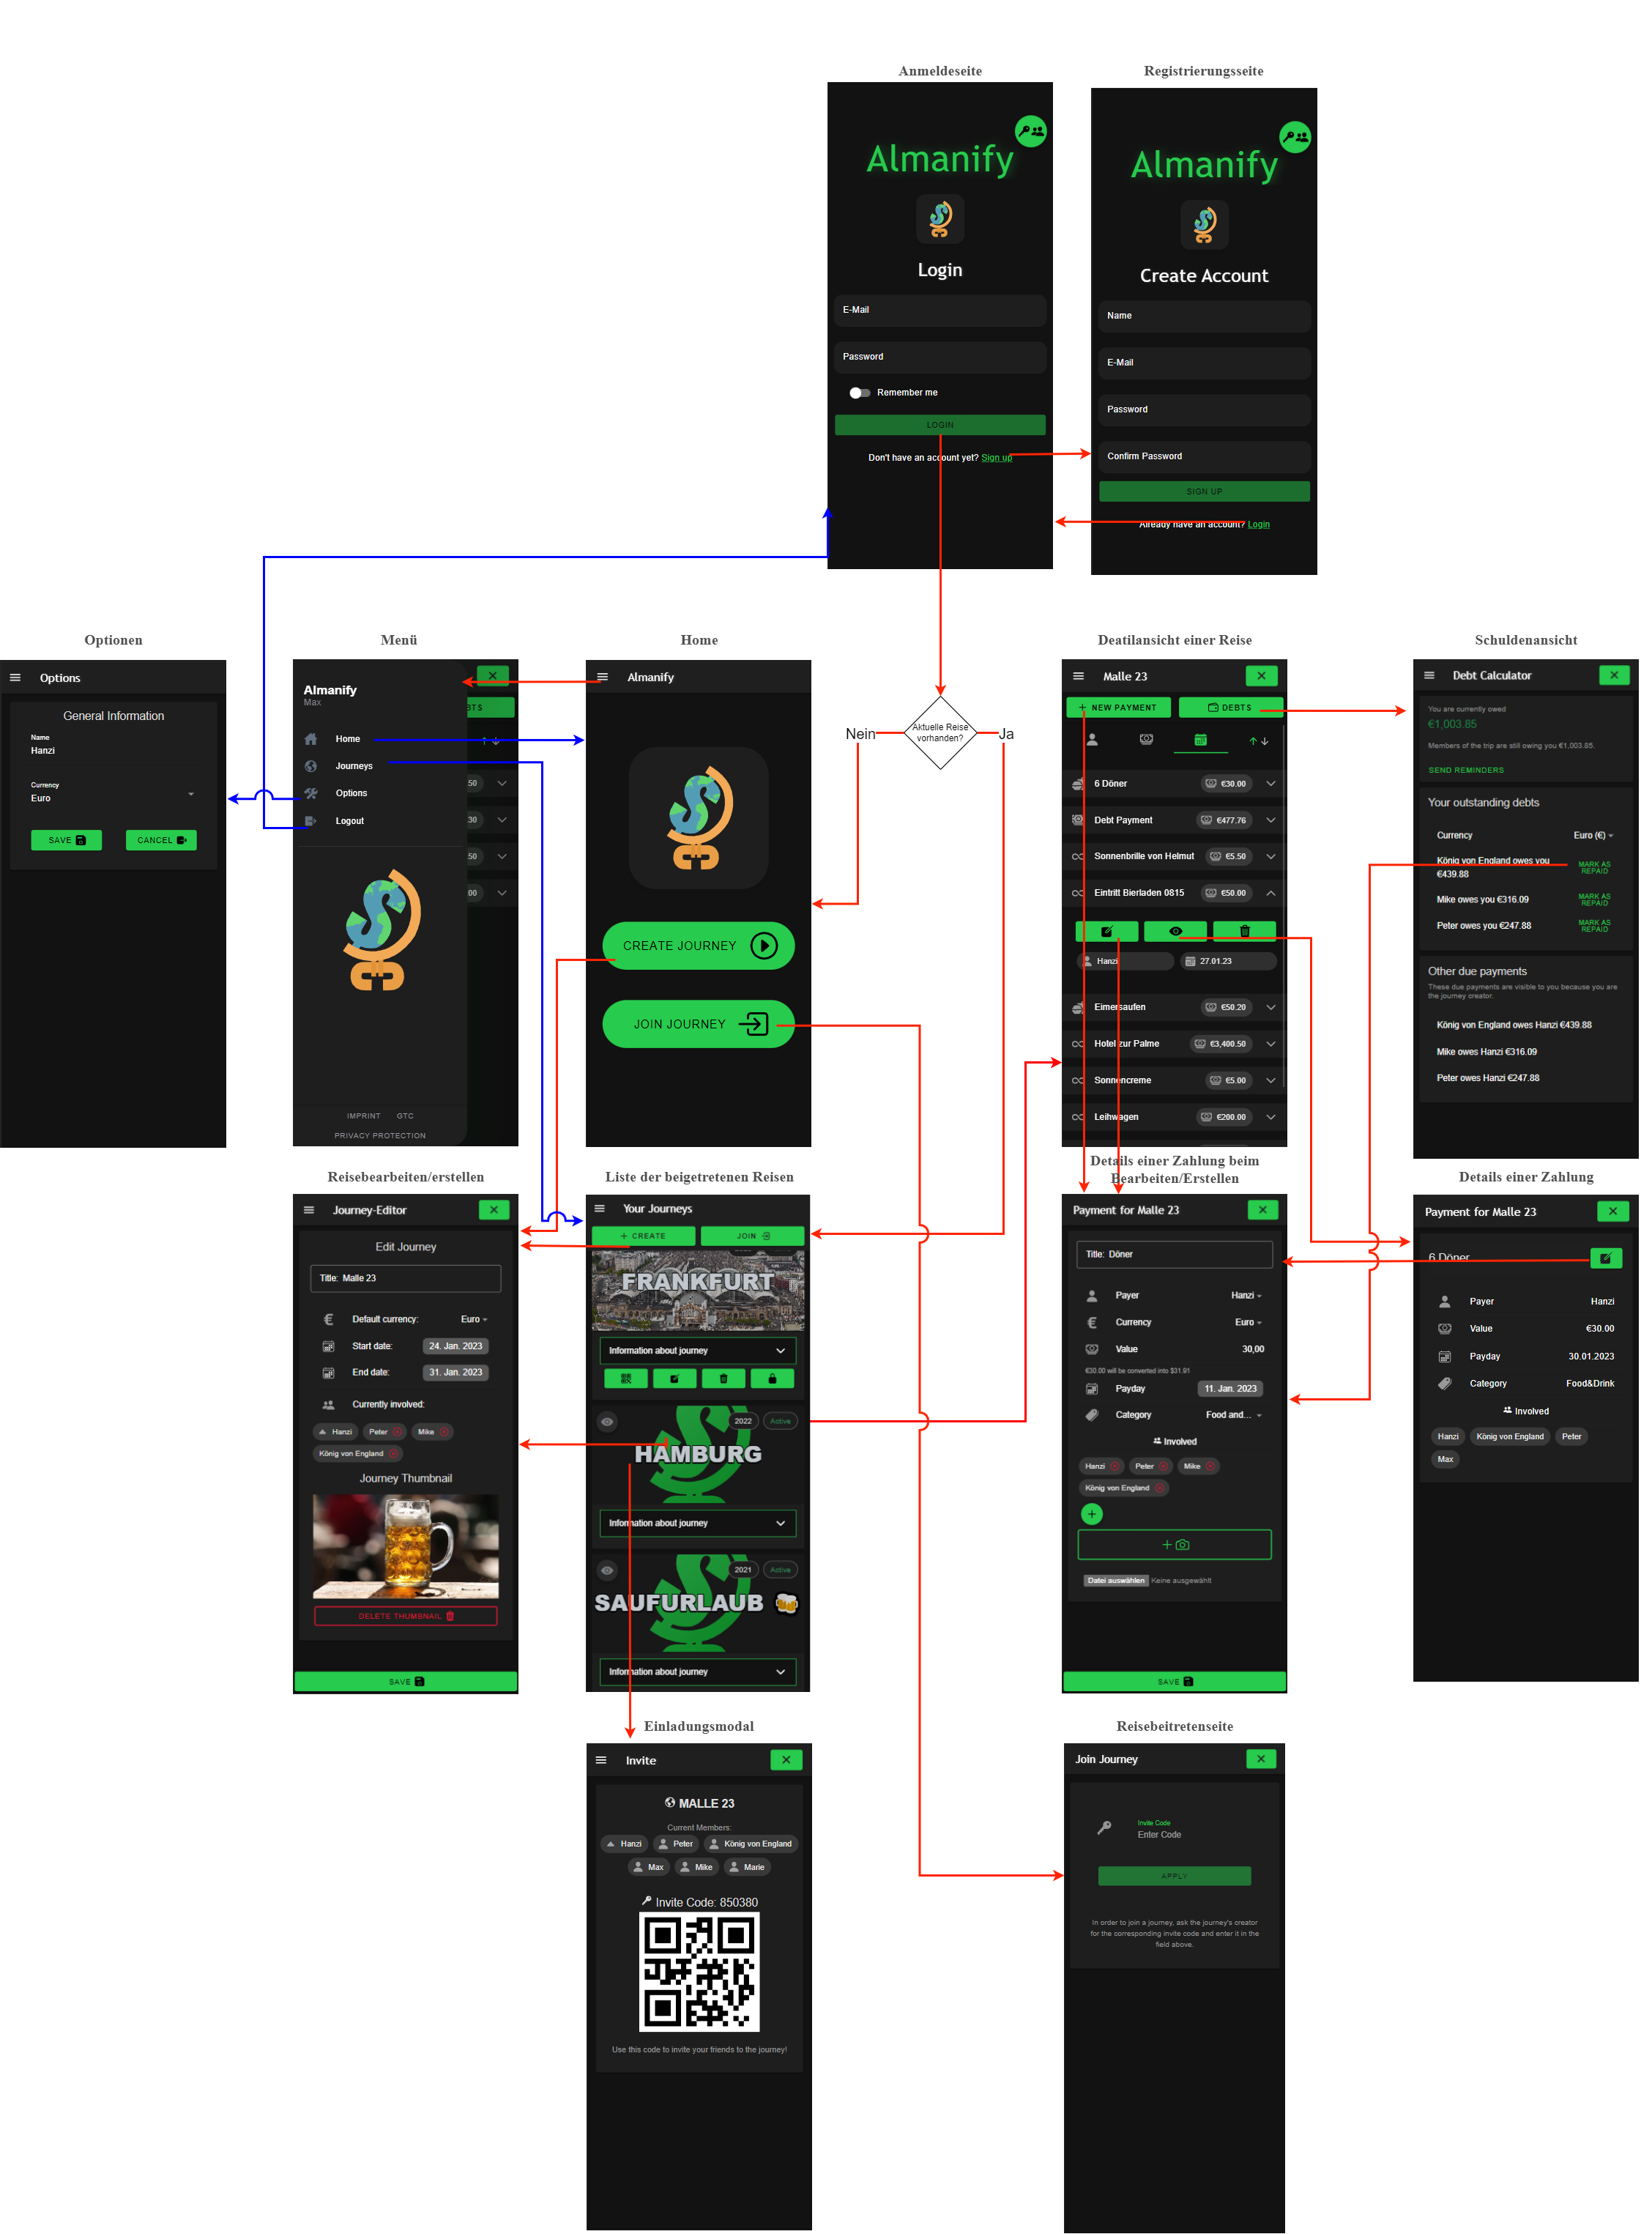
\includegraphics[width=\textwidth]{img/Sitemap}
	\caption[Sitemap]{Sitemap}
	%\captionsource{}
	\label{fig:Sitemap}
\end{figure}